\documentclass[aspectratio=43]{beamer}

\usetheme{Berlin}

\usepackage[utf8]{inputenc}
\usepackage[brazil]{babel}
\usepackage{graphicx}
\usepackage{hyperref}
\usepackage{listings}
\usepackage{tikz}

\lstset{
    basicstyle=\ttfamily\footnotesize,
    breaklines=true,
    frame=single,
    language=Lisp,
    keywordstyle=\color{blue},
    commentstyle=\color{green!60!black},
    stringstyle=\color{red},
    showstringspaces=false
}

\title{Recharging Robots PDDL Domain}
\subtitle{ICAPS - ipc2023}
\author{Bruno Ribeiro, Igor Penha \& Lucas Bergholz}
\institute{Universidade de Brasília}
\date{\today}

\begin{document}

\begin{frame}
  % \begin{tikzpicture}[remember picture,overlay]
  %   \node[opacity=0.1,inner sep=0pt] at (current page.center) {
  %     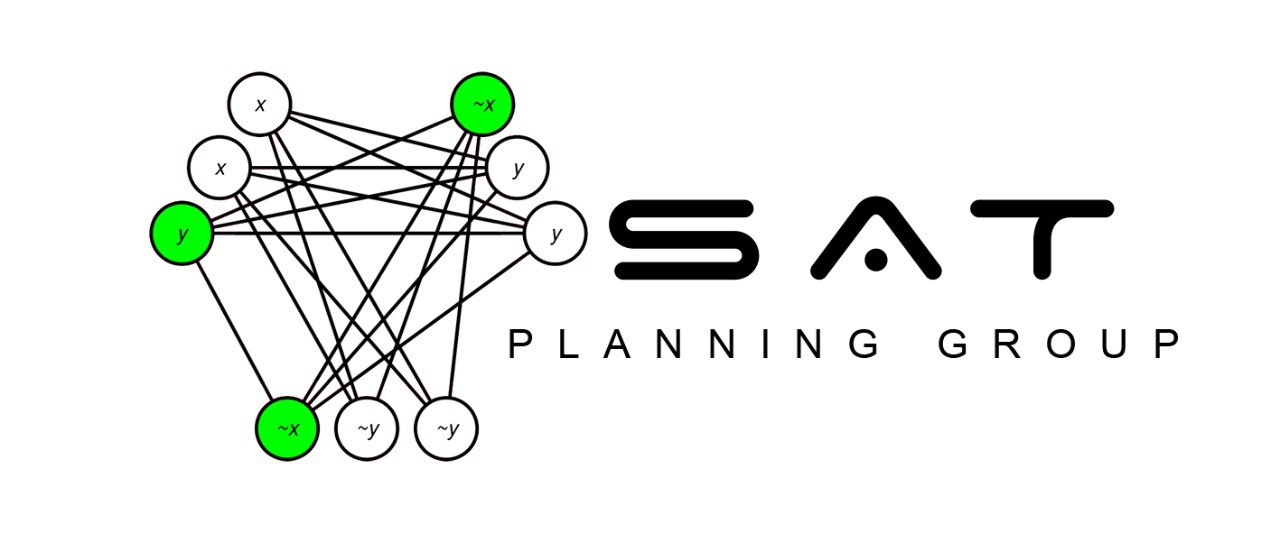
\includegraphics[width=10cm]{sat.jpg}
  %   };
  % \end{tikzpicture}
  \titlepage
\end{frame}

\begin{frame}{Sumário}
  \tableofcontents
\end{frame}

\section{Introdução}
\begin{frame}{Descrição do Domínio}
  \begin{itemize}
    \item Nome e características principais do domínio.
    \item Exemplos de problemas que ele resolve.
  \end{itemize}
\end{frame}

\section{Análise do Domínio}
\begin{frame}[allowframebreaks]{Análise do Domínio}
  \begin{itemize}
    \item Estrutura geral dos arquivos PDDL no domínio.
    \item Principais predicados e ações.
  \end{itemize}
  \vspace{1em}
  \lstinputlisting[language=Lisp,caption={Rechargin Robots PDDL Domain}]{domain.pddl}
\end{frame}

\section{Resultados}
\begin{frame}{Resultados}
  \begin{itemize}
    \item Casos de teste conduzidos.
    \item Desempenho e eficiência do domínio.
  \end{itemize}
\end{frame}

\section{Conclusões}
\begin{frame}{Conclusões}
  \begin{itemize}
    \item Discussão sobre os pontos fortes e fracos do domínio.
  \end{itemize}
\end{frame}

\begin{frame}{Obrigado!}
  \begin{center}
    Perguntas? \\
    \vspace{1cm}
    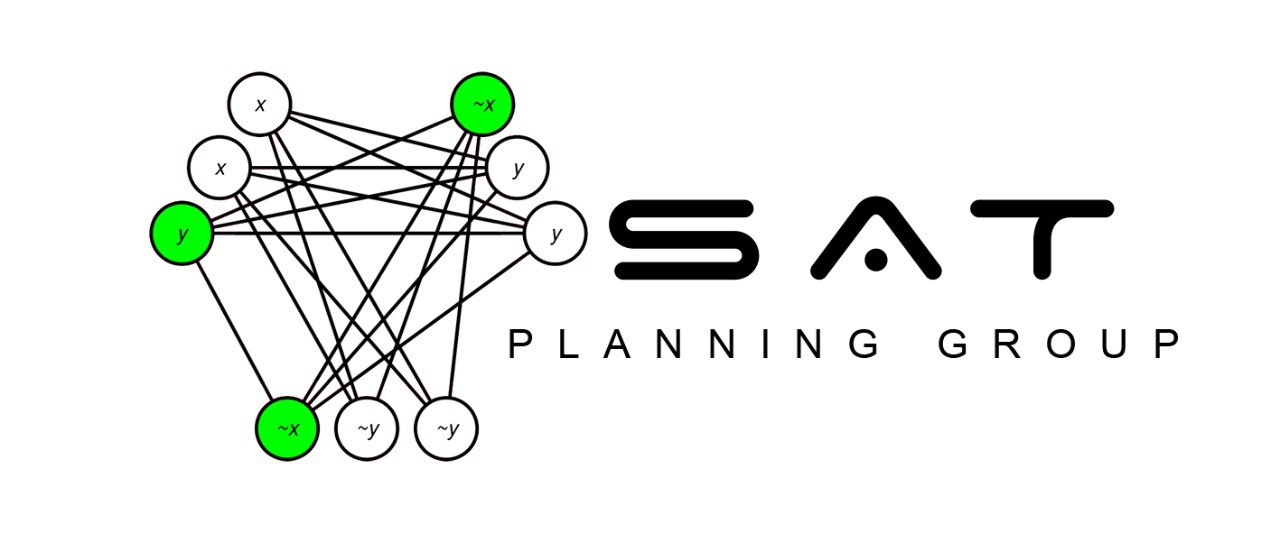
\includegraphics[width=0.3\textwidth]{sat.jpg}
  \end{center}
\end{frame}

\end{document}
